\PassOptionsToPackage{unicode=true}{hyperref} % options for packages loaded elsewhere
\PassOptionsToPackage{hyphens}{url}
%
\documentclass[]{book}
\usepackage{lmodern}
\usepackage{amssymb,amsmath}
\usepackage{ifxetex,ifluatex}
\usepackage{fixltx2e} % provides \textsubscript
\ifnum 0\ifxetex 1\fi\ifluatex 1\fi=0 % if pdftex
  \usepackage[T1]{fontenc}
  \usepackage[utf8]{inputenc}
  \usepackage{textcomp} % provides euro and other symbols
\else % if luatex or xelatex
  \usepackage{unicode-math}
  \defaultfontfeatures{Ligatures=TeX,Scale=MatchLowercase}
\fi
% use upquote if available, for straight quotes in verbatim environments
\IfFileExists{upquote.sty}{\usepackage{upquote}}{}
% use microtype if available
\IfFileExists{microtype.sty}{%
\usepackage[]{microtype}
\UseMicrotypeSet[protrusion]{basicmath} % disable protrusion for tt fonts
}{}
\IfFileExists{parskip.sty}{%
\usepackage{parskip}
}{% else
\setlength{\parindent}{0pt}
\setlength{\parskip}{6pt plus 2pt minus 1pt}
}
\usepackage{hyperref}
\hypersetup{
            pdftitle={Term project draft},
            pdfauthor={Kipling Klimas},
            pdfborder={0 0 0},
            breaklinks=true}
\urlstyle{same}  % don't use monospace font for urls
\usepackage{color}
\usepackage{fancyvrb}
\newcommand{\VerbBar}{|}
\newcommand{\VERB}{\Verb[commandchars=\\\{\}]}
\DefineVerbatimEnvironment{Highlighting}{Verbatim}{commandchars=\\\{\}}
% Add ',fontsize=\small' for more characters per line
\usepackage{framed}
\definecolor{shadecolor}{RGB}{248,248,248}
\newenvironment{Shaded}{\begin{snugshade}}{\end{snugshade}}
\newcommand{\AlertTok}[1]{\textcolor[rgb]{0.94,0.16,0.16}{#1}}
\newcommand{\AnnotationTok}[1]{\textcolor[rgb]{0.56,0.35,0.01}{\textbf{\textit{#1}}}}
\newcommand{\AttributeTok}[1]{\textcolor[rgb]{0.77,0.63,0.00}{#1}}
\newcommand{\BaseNTok}[1]{\textcolor[rgb]{0.00,0.00,0.81}{#1}}
\newcommand{\BuiltInTok}[1]{#1}
\newcommand{\CharTok}[1]{\textcolor[rgb]{0.31,0.60,0.02}{#1}}
\newcommand{\CommentTok}[1]{\textcolor[rgb]{0.56,0.35,0.01}{\textit{#1}}}
\newcommand{\CommentVarTok}[1]{\textcolor[rgb]{0.56,0.35,0.01}{\textbf{\textit{#1}}}}
\newcommand{\ConstantTok}[1]{\textcolor[rgb]{0.00,0.00,0.00}{#1}}
\newcommand{\ControlFlowTok}[1]{\textcolor[rgb]{0.13,0.29,0.53}{\textbf{#1}}}
\newcommand{\DataTypeTok}[1]{\textcolor[rgb]{0.13,0.29,0.53}{#1}}
\newcommand{\DecValTok}[1]{\textcolor[rgb]{0.00,0.00,0.81}{#1}}
\newcommand{\DocumentationTok}[1]{\textcolor[rgb]{0.56,0.35,0.01}{\textbf{\textit{#1}}}}
\newcommand{\ErrorTok}[1]{\textcolor[rgb]{0.64,0.00,0.00}{\textbf{#1}}}
\newcommand{\ExtensionTok}[1]{#1}
\newcommand{\FloatTok}[1]{\textcolor[rgb]{0.00,0.00,0.81}{#1}}
\newcommand{\FunctionTok}[1]{\textcolor[rgb]{0.00,0.00,0.00}{#1}}
\newcommand{\ImportTok}[1]{#1}
\newcommand{\InformationTok}[1]{\textcolor[rgb]{0.56,0.35,0.01}{\textbf{\textit{#1}}}}
\newcommand{\KeywordTok}[1]{\textcolor[rgb]{0.13,0.29,0.53}{\textbf{#1}}}
\newcommand{\NormalTok}[1]{#1}
\newcommand{\OperatorTok}[1]{\textcolor[rgb]{0.81,0.36,0.00}{\textbf{#1}}}
\newcommand{\OtherTok}[1]{\textcolor[rgb]{0.56,0.35,0.01}{#1}}
\newcommand{\PreprocessorTok}[1]{\textcolor[rgb]{0.56,0.35,0.01}{\textit{#1}}}
\newcommand{\RegionMarkerTok}[1]{#1}
\newcommand{\SpecialCharTok}[1]{\textcolor[rgb]{0.00,0.00,0.00}{#1}}
\newcommand{\SpecialStringTok}[1]{\textcolor[rgb]{0.31,0.60,0.02}{#1}}
\newcommand{\StringTok}[1]{\textcolor[rgb]{0.31,0.60,0.02}{#1}}
\newcommand{\VariableTok}[1]{\textcolor[rgb]{0.00,0.00,0.00}{#1}}
\newcommand{\VerbatimStringTok}[1]{\textcolor[rgb]{0.31,0.60,0.02}{#1}}
\newcommand{\WarningTok}[1]{\textcolor[rgb]{0.56,0.35,0.01}{\textbf{\textit{#1}}}}
\usepackage{longtable,booktabs}
% Fix footnotes in tables (requires footnote package)
\IfFileExists{footnote.sty}{\usepackage{footnote}\makesavenoteenv{longtable}}{}
\usepackage{graphicx,grffile}
\makeatletter
\def\maxwidth{\ifdim\Gin@nat@width>\linewidth\linewidth\else\Gin@nat@width\fi}
\def\maxheight{\ifdim\Gin@nat@height>\textheight\textheight\else\Gin@nat@height\fi}
\makeatother
% Scale images if necessary, so that they will not overflow the page
% margins by default, and it is still possible to overwrite the defaults
% using explicit options in \includegraphics[width, height, ...]{}
\setkeys{Gin}{width=\maxwidth,height=\maxheight,keepaspectratio}
\setlength{\emergencystretch}{3em}  % prevent overfull lines
\providecommand{\tightlist}{%
  \setlength{\itemsep}{0pt}\setlength{\parskip}{0pt}}
\setcounter{secnumdepth}{5}
% Redefines (sub)paragraphs to behave more like sections
\ifx\paragraph\undefined\else
\let\oldparagraph\paragraph
\renewcommand{\paragraph}[1]{\oldparagraph{#1}\mbox{}}
\fi
\ifx\subparagraph\undefined\else
\let\oldsubparagraph\subparagraph
\renewcommand{\subparagraph}[1]{\oldsubparagraph{#1}\mbox{}}
\fi

% set default figure placement to htbp
\makeatletter
\def\fps@figure{htbp}
\makeatother

\usepackage{booktabs}
\usepackage[]{natbib}
\bibliographystyle{apalike}

\title{Term project draft}
\author{Kipling Klimas}
\date{2021-04-30}

\begin{document}
\maketitle

{
\setcounter{tocdepth}{1}
\tableofcontents
}
\hypertarget{introduction}{%
\chapter{Introduction}\label{introduction}}

This project is focused on the relationship between a variety of environmental, topographic and derived variables and burn severity data for forest and non-forest environments in Utah.

Burn severity is a measure of ecological change after wildfire, commonly assessed in terms of vegetation mortality or biomass loss,
and is burn severity data is easily collected through remote sensing. Burn severity data is available from the The Monitoring Trends in Burn Severity (MTBS) databas, which containes burn severity data for wildfires \textgreater{}1000 acres across the continental US.
These data are available in the form of spatially explicit raster layers with continuous and categorical burn severity layers.

The database used in this project contains fire behavior, structure, topographic, risk and vegetation `predictor' variables for both
forest and non-forest land along with burn severity data.

\hypertarget{project-goals}{%
\section{Project goals}\label{project-goals}}

The specific goal of this project is to vizualize the relationship between burn severity and a variety of environmental variables in forest and non-forest enviornments. This includes creating plots that show:

\begin{enumerate}
\def\labelenumi{\arabic{enumi}.}
\tightlist
\item
  Burn severity vs.~elevation
\item
  Burn severity vs.~canopy categories
\item
  Burn severity vs.~Vegetation type
\item
  Burn severity vs.~elevation with risk and canopy variables overlayed
\end{enumerate}

\hypertarget{project-outline}{%
\section{Project outline}\label{project-outline}}

The book is composed of the following chapters:

\begin{itemize}
\tightlist
\item
  Chapter 1: data description and structure
\item
  Chapter 2: database creation
\item
  Chapter 3: database connection'
\item
  Chapter 4: forest data visualization
\item
  Chapter 5: non-forest data visualization
\end{itemize}

\hypertarget{data}{%
\chapter{Data description and database structure}\label{data}}

Forest strcuture, topographic, and environmental variables are needed to create a machine learning model training dataset.

\begin{center}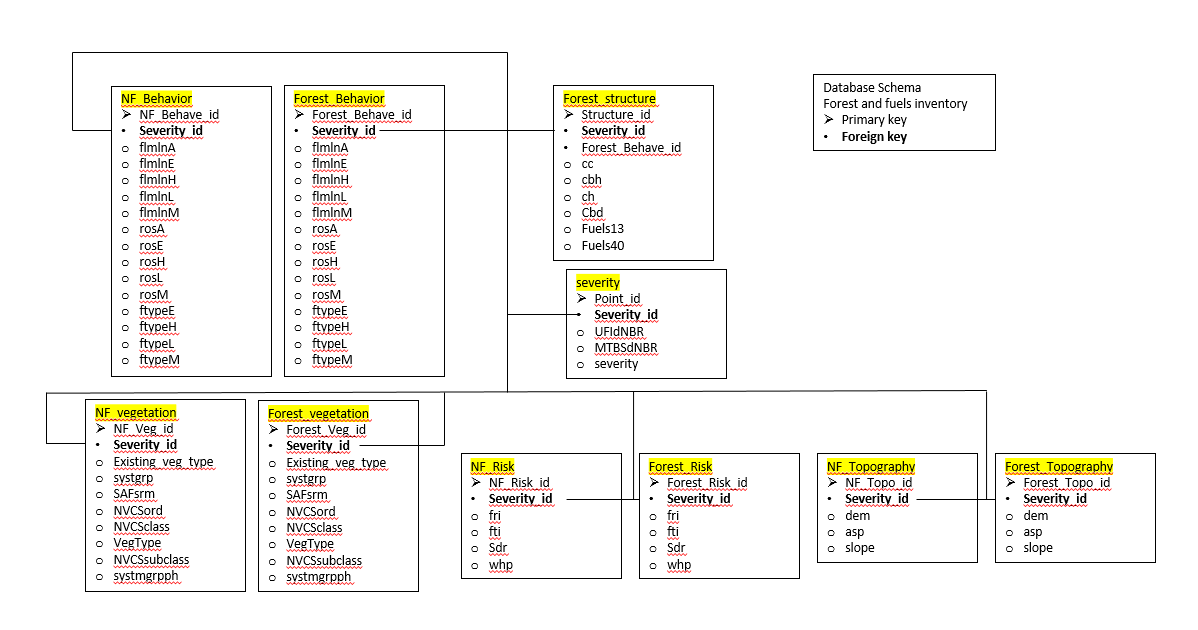
\includegraphics{db_structure} \end{center}

Figure 1: databse structure for fire severity databse.

This database contains tables for fire behavior, risk, topographic, vegetation and structural variables extracted from spatially explicit raster data layers for use as a training dataset in RandomForest (RF) models.

The tables are linked to the severity table by the foreign key `severity\_id' which keeps track of both forest and non-forest severity datapoints. This database structure also allows data visualization between forest and non-forest landcover in Utah.

\hypertarget{creation}{%
\chapter{Database creation}\label{creation}}

Start

Install and open packages \texttt{RSQLite}

\begin{Shaded}
\begin{Highlighting}[]
\KeywordTok{install.packages}\NormalTok{(}\StringTok{"RSQLite"}\NormalTok{)}
\KeywordTok{library}\NormalTok{(RSQLite)}
\end{Highlighting}
\end{Shaded}

Establish database connection

Connecting to the term\_project database

\begin{Shaded}
\begin{Highlighting}[]
\NormalTok{term_project <-}\StringTok{ }\KeywordTok{dbConnect}\NormalTok{(}\DataTypeTok{drv =}\NormalTok{ RSQLite}\OperatorTok{::}\KeywordTok{SQLite}\NormalTok{(),}
                        \StringTok{"C:/Users/A02345823/Box/Lab_Group/Kipling/Classes/WILD6900_EcoRepSci/Term_project/Term_project/database/severity.db"}\NormalTok{)}
\end{Highlighting}
\end{Shaded}

Create severity table
Term project database creation based on structure in figure 1

\begin{Shaded}
\begin{Highlighting}[]
\KeywordTok{dbExecute}\NormalTok{(term_project, }\StringTok{"CREATE TABLE severity(}
\StringTok{severity_id integer NOT NULL PRIMARY KEY,}
\StringTok{MTBSdNBR float,}
\StringTok{severity float}
\StringTok{);"}\NormalTok{)}
\end{Highlighting}
\end{Shaded}

Create forest behavior table

\begin{Shaded}
\begin{Highlighting}[]
\KeywordTok{dbExecute}\NormalTok{(term_project, }\StringTok{"CREATE TABLE forest_behavior(}
\StringTok{forest_behave_id integer NOT NULL PRIMARY KEY,}
\StringTok{severity_id float,}
\StringTok{flmlnA float,}
\StringTok{flmlnE float,}
\StringTok{flmlnH float,}
\StringTok{flmlnL float,}
\StringTok{flmlnM float,}
\StringTok{ftype_E float,}
\StringTok{ftype_H float,}
\StringTok{ftype_L float,}
\StringTok{ftype_M float,}
\StringTok{ros float,}
\StringTok{rosE float,}
\StringTok{rosH float,}
\StringTok{rosL float,}
\StringTok{rosM float,}
\StringTok{FOREIGN KEY(severity_id) REFERENCES severity(severity_id)}
\StringTok{);"}\NormalTok{)}
\end{Highlighting}
\end{Shaded}

Create forest risk table

\begin{Shaded}
\begin{Highlighting}[]
\KeywordTok{dbExecute}\NormalTok{(term_project, }\StringTok{"CREATE TABLE forest_risk(}
\StringTok{forest_risk_id integer NOT NULL PRIMARY KEY,}
\StringTok{severity_id float,}
\StringTok{fri float,}
\StringTok{fti float,}
\StringTok{sdr varchar(12),}
\StringTok{WHP float,}
\StringTok{FOREIGN KEY(severity_id) REFERENCES severity(severity_id)}
\StringTok{);"}\NormalTok{)}
\end{Highlighting}
\end{Shaded}

Create forest\_structure table

\begin{Shaded}
\begin{Highlighting}[]
\KeywordTok{dbExecute}\NormalTok{(term_project, }\StringTok{"CREATE TABLE forest_structure(}
\StringTok{str_id integer NOT NULL PRIMARY KEY,}
\StringTok{severity_id float,}
\StringTok{wwacbd float,}
\StringTok{wwacbh float,}
\StringTok{wwacc float,}
\StringTok{wwach float,}
\StringTok{wwafuel13 float,}
\StringTok{wwafuel40 float,}
\StringTok{FOREIGN KEY(severity_id) REFERENCES severity(severity_id)}
\StringTok{);"}\NormalTok{)}
\end{Highlighting}
\end{Shaded}

Create forest\_topo table

\begin{Shaded}
\begin{Highlighting}[]
\KeywordTok{dbExecute}\NormalTok{(term_project, }\StringTok{"CREATE TABLE forest_topo(}
\StringTok{forest_topo_id integer NOT NULL PRIMARY KEY,}
\StringTok{severity_id float,}
\StringTok{asp varchar(5),}
\StringTok{dem float,}
\StringTok{slope float,}
\StringTok{FOREIGN KEY(severity_id) REFERENCES severity(severity_id)}
\StringTok{);"}\NormalTok{)}
\end{Highlighting}
\end{Shaded}

Create forest\_veg table

\begin{Shaded}
\begin{Highlighting}[]
\KeywordTok{dbExecute}\NormalTok{(term_project, }\StringTok{"CREATE TABLE forest_veg(}
\StringTok{forest_veg_id integer NOT NULL PRIMARY KEY,}
\StringTok{severity_id float,}
\StringTok{EVT varchar(60),}
\StringTok{SystGrp varchar(60),}
\StringTok{SAFSrm varchar(60),}
\StringTok{NVCSOrd varchar(16),}
\StringTok{NVCSclass varchar(25),}
\StringTok{NVCSsubclass varchar(40),}
\StringTok{SYSTMGRPPH varchar(30),}
\StringTok{FOREIGN KEY(severity_id) REFERENCES severity(severity_id)}
\StringTok{);"}\NormalTok{)}
\end{Highlighting}
\end{Shaded}

Create non-forest db tables

Create non-forest behavior table

\begin{Shaded}
\begin{Highlighting}[]
\KeywordTok{dbExecute}\NormalTok{(term_project, }\StringTok{"CREATE TABLE nf_behavior(}
\StringTok{nf_behave_id integer NOT NULL PRIMARY KEY,}
\StringTok{severity_id float,}
\StringTok{flmlnA float,}
\StringTok{flmlnE float,}
\StringTok{flmlnH float,}
\StringTok{flmlnL float,}
\StringTok{flmlnM float,}
\StringTok{ftype_E float,}
\StringTok{ftype_H float,}
\StringTok{ftype_L float,}
\StringTok{ftype_M float,}
\StringTok{ros float,}
\StringTok{rosE float,}
\StringTok{rosH float,}
\StringTok{rosL float,}
\StringTok{rosM float,}
\StringTok{FOREIGN KEY(severity_id) REFERENCES severity(severity_id)}
\StringTok{);"}\NormalTok{)}
\end{Highlighting}
\end{Shaded}

Create non-forest risk table

\begin{Shaded}
\begin{Highlighting}[]
\KeywordTok{dbExecute}\NormalTok{(term_project, }\StringTok{"CREATE TABLE nf_risk(}
\StringTok{nf_risk_id integer NOT NULL PRIMARY KEY,}
\StringTok{severity_id float,}
\StringTok{fri float,}
\StringTok{fti float,}
\StringTok{sdr varchar(12),}
\StringTok{WHP float,}
\StringTok{FOREIGN KEY(severity_id) REFERENCES severity(severity_id)}
\StringTok{);"}\NormalTok{)}
\end{Highlighting}
\end{Shaded}

Create non-forest\_structure table

\begin{Shaded}
\begin{Highlighting}[]
\KeywordTok{dbExecute}\NormalTok{(term_project, }\StringTok{"CREATE TABLE nf_structure(}
\StringTok{nf_str_id integer NOT NULL PRIMARY KEY,}
\StringTok{severity_id float,}
\StringTok{wwacbd float,}
\StringTok{wwacbh float,}
\StringTok{wwacc float,}
\StringTok{wwach float,}
\StringTok{wwafuel13 float,}
\StringTok{wwafuel40 float,}
\StringTok{FOREIGN KEY(severity_id) REFERENCES severity(severity_id)}
\StringTok{);"}\NormalTok{)}
\end{Highlighting}
\end{Shaded}

Create non-forest\_topo table

\begin{Shaded}
\begin{Highlighting}[]
\KeywordTok{dbExecute}\NormalTok{(term_project, }\StringTok{"CREATE TABLE nf_topo(}
\StringTok{nf_topo_id integer NOT NULL PRIMARY KEY,}
\StringTok{severity_id float,}
\StringTok{asp varchar(5),}
\StringTok{dem float,}
\StringTok{slope float,}
\StringTok{FOREIGN KEY(severity_id) REFERENCES severity(severity_id)}
\StringTok{);"}\NormalTok{)}
\end{Highlighting}
\end{Shaded}

Create non-forest\_veg table

\begin{Shaded}
\begin{Highlighting}[]
\KeywordTok{dbExecute}\NormalTok{(term_project, }\StringTok{"CREATE TABLE nf_veg(}
\StringTok{nf_veg_id integer NOT NULL PRIMARY KEY,}
\StringTok{severity_id float,}
\StringTok{EVT varchar(60),}
\StringTok{SystGrp varchar(60),}
\StringTok{SAFSrm varchar(60),}
\StringTok{NVCSOrd varchar(16),}
\StringTok{NVCSclass varchar(25),}
\StringTok{NVCSsubclass varchar(40),}
\StringTok{SYSTMGRPPH varchar(30),}
\StringTok{FOREIGN KEY(severity_id) REFERENCES severity(severity_id)}
\StringTok{);"}\NormalTok{)}
\end{Highlighting}
\end{Shaded}

\hypertarget{SQL}{%
\chapter{Database connection}\label{SQL}}

Start

Install package \texttt{RSQLite}

\begin{Shaded}
\begin{Highlighting}[]
\KeywordTok{install.packages}\NormalTok{(}\StringTok{"RSQLite"}\NormalTok{)}
\KeywordTok{library}\NormalTok{(RSQLite)}
\end{Highlighting}
\end{Shaded}

Establish datebase connection and create tables

\begin{Shaded}
\begin{Highlighting}[]
\NormalTok{severity_db <-}\StringTok{ }\KeywordTok{dbConnect}\NormalTok{(}\DataTypeTok{drv =}\NormalTok{ RSQLite}\OperatorTok{::}\KeywordTok{SQLite}\NormalTok{(),}
                \StringTok{"/Users/kiplingklimas/Box/Lab_Group/Kipling/Classes/WILD6900_EcoRepSci/Term_project/Term_project/database/severity.db"}\NormalTok{)}

\NormalTok{severity <-}\StringTok{ }\KeywordTok{dbGetQuery}\NormalTok{(severity_db, }\StringTok{"SELECT * FROM severity;"}\NormalTok{)}
\NormalTok{forest_behavior <-}\StringTok{ }\KeywordTok{dbGetQuery}\NormalTok{(severity_db, }\StringTok{"SELECT * FROM forest_behavior;"}\NormalTok{)}
\NormalTok{forest_risk <-}\StringTok{ }\KeywordTok{dbGetQuery}\NormalTok{(severity_db, }\StringTok{"SELECT * FROM forest_risk;"}\NormalTok{)}
\NormalTok{forest_structure <-}\StringTok{ }\KeywordTok{dbGetQuery}\NormalTok{(severity_db, }\StringTok{"SELECT * FROM forest_structure;"}\NormalTok{)}
\NormalTok{forest_topo <-}\StringTok{ }\KeywordTok{dbGetQuery}\NormalTok{(severity_db, }\StringTok{"SELECT * FROM forest_topo;"}\NormalTok{)}
\NormalTok{forest_veg <-}\StringTok{ }\KeywordTok{dbGetQuery}\NormalTok{(severity_db, }\StringTok{"SELECT * FROM forest_veg;"}\NormalTok{)}
\NormalTok{nf_behavior <-}\StringTok{ }\KeywordTok{dbGetQuery}\NormalTok{(severity_db, }\StringTok{"SELECT * FROM nf_behavior;"}\NormalTok{)}
\NormalTok{nf_risk <-}\StringTok{ }\KeywordTok{dbGetQuery}\NormalTok{(severity_db, }\StringTok{"SELECT * FROM nf_risk;"}\NormalTok{)}
\NormalTok{nf_structure <-}\StringTok{ }\KeywordTok{dbGetQuery}\NormalTok{(severity_db, }\StringTok{"SELECT * FROM nf_structure;"}\NormalTok{)}
\NormalTok{nf_topo <-}\StringTok{ }\KeywordTok{dbGetQuery}\NormalTok{(severity_db, }\StringTok{"SELECT * FROM nf_topo;"}\NormalTok{)}
\NormalTok{nf_veg <-}\StringTok{ }\KeywordTok{dbGetQuery}\NormalTok{(severity_db, }\StringTok{"SELECT * FROM nf_veg;"}\NormalTok{)}
\end{Highlighting}
\end{Shaded}

This is fire severity dataset shows the relationship between severity measurements and a variety of predictive variables
including topographic, vegetation, structural and derived risk indices.
Data was differentiated between forest and non-forest points to compare severity relationships between forests and non-forest
landcover systems.

\hypertarget{dataviz}{%
\chapter{Forest data visualization}\label{dataviz}}

Install packages \texttt{tidyverse}, \texttt{viridis} and \texttt{ggridges}

\begin{verbatim}
## -- Attaching packages --------------------------------------- tidyverse 1.3.1 --
\end{verbatim}

\begin{verbatim}
## v ggplot2 3.3.3     v purrr   0.3.4
## v tibble  3.1.1     v dplyr   1.0.5
## v tidyr   1.1.3     v stringr 1.4.0
## v readr   1.4.0     v forcats 0.5.1
\end{verbatim}

\begin{verbatim}
## -- Conflicts ------------------------------------------ tidyverse_conflicts() --
## x dplyr::filter() masks stats::filter()
## x dplyr::lag()    masks stats::lag()
\end{verbatim}

\begin{verbatim}
## Loading required package: viridisLite
\end{verbatim}

\begin{Shaded}
\begin{Highlighting}[]
\NormalTok{sev <-}\StringTok{ }\NormalTok{forest_topo }\OperatorTok\StringTok{ }
\StringTok{  }\KeywordTok{left_join}\NormalTok{(severity, }\DataTypeTok{by =} \StringTok{"severity_id"}\NormalTok{) }\OperatorTok\StringTok{ }
\StringTok{  }\KeywordTok{select}\NormalTok{(dem, severity)}

\NormalTok{reg <-}\StringTok{ }\KeywordTok{lm}\NormalTok{(}\DataTypeTok{formula=}\NormalTok{ severity }\OperatorTok{~}\StringTok{ }\NormalTok{dem, }\DataTypeTok{data =}\NormalTok{ sev)}
\NormalTok{regs <-}\StringTok{ }\KeywordTok{predict}\NormalTok{(reg, }\DataTypeTok{se.fit =} \OtherTok{TRUE}\NormalTok{)}
\NormalTok{regs <-}\StringTok{ }\KeywordTok{data.frame}\NormalTok{(}\DataTypeTok{mean =}\NormalTok{ regs}\OperatorTok{$}\NormalTok{fit,}
                    \DataTypeTok{upr =}\NormalTok{ regs}\OperatorTok{$}\NormalTok{fit }\OperatorTok{+}\StringTok{ }\FloatTok{1.96} \OperatorTok{*}\StringTok{ }\NormalTok{regs}\OperatorTok{$}\NormalTok{se.fit,}
                    \DataTypeTok{lwr =}\NormalTok{ regs}\OperatorTok{$}\NormalTok{fit }\OperatorTok{-}\StringTok{ }\FloatTok{1.96} \OperatorTok{*}\StringTok{ }\NormalTok{regs}\OperatorTok{$}\NormalTok{se.fit)}
            

\NormalTok{forest_topo }\OperatorTok\StringTok{ }
\StringTok{  }\KeywordTok{left_join}\NormalTok{(severity, }\DataTypeTok{by =} \StringTok{"severity_id"}\NormalTok{) }\OperatorTok\StringTok{ }
\StringTok{  }\KeywordTok{select}\NormalTok{(dem, severity) }\OperatorTok\StringTok{ }
\StringTok{  }\KeywordTok{ggplot}\NormalTok{(}\KeywordTok{aes}\NormalTok{(}\DataTypeTok{x =}\NormalTok{ dem, }\DataTypeTok{y =}\NormalTok{ severity, }\DataTypeTok{color=}\NormalTok{ dem)) }\OperatorTok{+}
\StringTok{  }\KeywordTok{geom_point}\NormalTok{(}\DataTypeTok{alpha =} \FloatTok{0.5}\NormalTok{) }\OperatorTok{+}
\StringTok{  }\KeywordTok{scale_color_viridis_c}\NormalTok{(}\DataTypeTok{option =} \StringTok{"magma"}\NormalTok{) }\OperatorTok{+}
\StringTok{  }\KeywordTok{geom_line}\NormalTok{(}\KeywordTok{aes}\NormalTok{(}\DataTypeTok{y =}\NormalTok{ regs}\OperatorTok{$}\NormalTok{mean, }\DataTypeTok{color =}\NormalTok{ regs}\OperatorTok{$}\NormalTok{mean)) }\OperatorTok{+}
\StringTok{  }\KeywordTok{labs}\NormalTok{(}\DataTypeTok{y =} \StringTok{"Severity (dNBR)"}\NormalTok{, }\DataTypeTok{x =} \StringTok{"Elevation (m)"}\NormalTok{) }\OperatorTok{+}
\StringTok{  }\KeywordTok{theme_light}\NormalTok{() }
\end{Highlighting}
\end{Shaded}

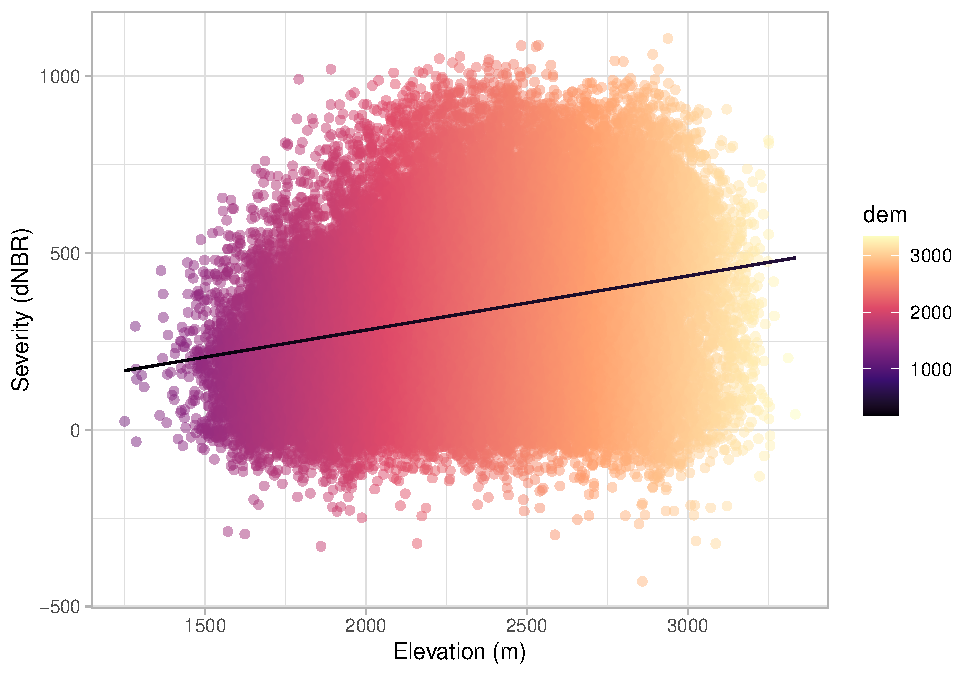
\includegraphics{term_project_files/figure-latex/f_simple_plots-1.pdf}

Simple scatter plot of forest severity vs.~elevation (m)

\begin{Shaded}
\begin{Highlighting}[]
\NormalTok{forest_behavior }\OperatorTok\StringTok{ }
\StringTok{  }\KeywordTok{left_join}\NormalTok{(severity, }\DataTypeTok{by =} \StringTok{"severity_id"}\NormalTok{) }\OperatorTok\StringTok{ }
\StringTok{  }\KeywordTok{mutate}\NormalTok{(}\DataTypeTok{ftypeE =} \KeywordTok{case_when}\NormalTok{(}
\NormalTok{    ftype_E }\OperatorTok{==}\StringTok{ }\DecValTok{3} \OperatorTok{~}\StringTok{ "Surface"}\NormalTok{,}
\NormalTok{    ftype_E }\OperatorTok{==}\StringTok{ }\DecValTok{4} \OperatorTok{~}\StringTok{ "Passive"}\NormalTok{,}
\NormalTok{    ftype_E }\OperatorTok{==}\StringTok{ }\DecValTok{5} \OperatorTok{~}\StringTok{ "Passive"}\NormalTok{,}
\NormalTok{    ftype_E }\OperatorTok{==}\StringTok{ }\DecValTok{6} \OperatorTok{~}\StringTok{ "Active"}\NormalTok{,}
\NormalTok{    ftype_E }\OperatorTok{==}\StringTok{ }\DecValTok{7} \OperatorTok{~}\StringTok{ "Active"}\NormalTok{,}
\NormalTok{  )) }\OperatorTok\StringTok{ }
\StringTok{  }\KeywordTok{ggplot}\NormalTok{(}\KeywordTok{aes}\NormalTok{(}\DataTypeTok{y =}\NormalTok{ ftypeE, }\DataTypeTok{x =}\NormalTok{ severity, }\DataTypeTok{fill =}\NormalTok{ ftypeE)) }\OperatorTok{+}
\StringTok{  }\NormalTok{ggridges}\OperatorTok{::}\KeywordTok{geom_density_ridges}\NormalTok{(}\DataTypeTok{scale =} \DecValTok{8}\NormalTok{, }\DataTypeTok{alpha =} \FloatTok{0.5}\NormalTok{, }\DataTypeTok{show.legend =} \OtherTok{FALSE}\NormalTok{) }\OperatorTok{+}
\StringTok{  }\KeywordTok{theme}\NormalTok{(}\DataTypeTok{axis.text.x =} \KeywordTok{element_text}\NormalTok{(}\DataTypeTok{angle =} \DecValTok{45}\NormalTok{, }\DataTypeTok{hjust =} \DecValTok{1}\NormalTok{))  }\OperatorTok{+}
\StringTok{  }\KeywordTok{labs}\NormalTok{(}\DataTypeTok{y =} \StringTok{"Fire type Extreme"}\NormalTok{, }\DataTypeTok{x =} \StringTok{"Severity"}\NormalTok{) }\OperatorTok{+}
\StringTok{  }\KeywordTok{scale_color_viridis_d}\NormalTok{(}\DataTypeTok{option =} \StringTok{"magma"}\NormalTok{) }\OperatorTok{+}
\StringTok{  }\KeywordTok{theme_minimal}\NormalTok{()}
\end{Highlighting}
\end{Shaded}

\begin{verbatim}
## Picking joint bandwidth of 29.2
\end{verbatim}

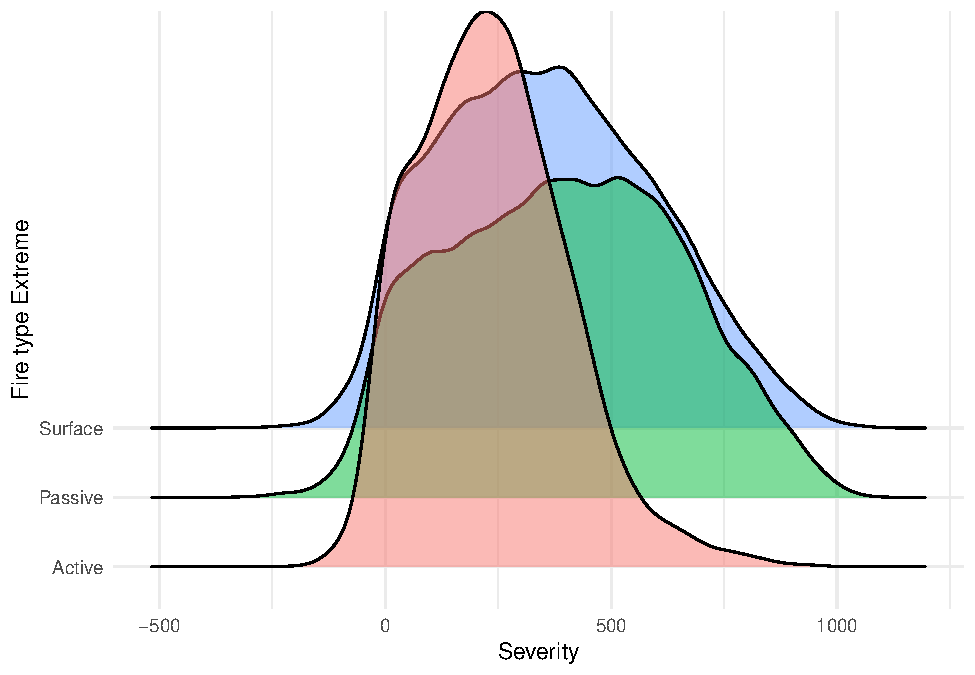
\includegraphics{term_project_files/figure-latex/behavior-1.pdf}

Density curves of fire type extreme by severity
The variable FtypeE represents the fire type under extreme (99 percentile) weather scenarios.
The three `types' of fire in described by this variable are:
1. Surface - fire that burns surface fuels
2. Passive - fire that burns both surface and intermediate ladder fuels
3. Active - fire that burns in the canopy of the forest

This density plot is of interest because it shows that Active fire type represents lower severity burned areas than
Surface or Passive, which is contrary to a popular assumption that crown/canopy fire is associated with high-severity
burned areas.

\begin{Shaded}
\begin{Highlighting}[]
\NormalTok{forest_veg }\OperatorTok\StringTok{ }
\StringTok{  }\KeywordTok{left_join}\NormalTok{(severity, }\DataTypeTok{by =} \StringTok{"severity_id"}\NormalTok{) }\OperatorTok\StringTok{ }
\StringTok{  }\KeywordTok{filter}\NormalTok{(}\OperatorTok{!}\KeywordTok{is.na}\NormalTok{(severity_id)) }\OperatorTok\StringTok{ }
\StringTok{  }\KeywordTok{ggplot}\NormalTok{(}\KeywordTok{aes}\NormalTok{(}\DataTypeTok{x =}\NormalTok{ NVCSsubclass, }\DataTypeTok{y =}\NormalTok{ severity)) }\OperatorTok{+}
\StringTok{  }\KeywordTok{geom_boxplot}\NormalTok{() }\OperatorTok{+}
\StringTok{  }\KeywordTok{labs}\NormalTok{(}\DataTypeTok{y =} \StringTok{"Severity (dNBR)"}\NormalTok{, }\DataTypeTok{x =} \StringTok{"Canopy type"}\NormalTok{) }\OperatorTok{+}
\StringTok{  }\KeywordTok{theme_bw}\NormalTok{() }\OperatorTok{+}
\StringTok{  }\KeywordTok{theme}\NormalTok{(}\DataTypeTok{axis.text.x =} \KeywordTok{element_text}\NormalTok{(}\DataTypeTok{angle =} \DecValTok{45}\NormalTok{, }\DataTypeTok{hjust =} \DecValTok{1}\NormalTok{)) }
\end{Highlighting}
\end{Shaded}

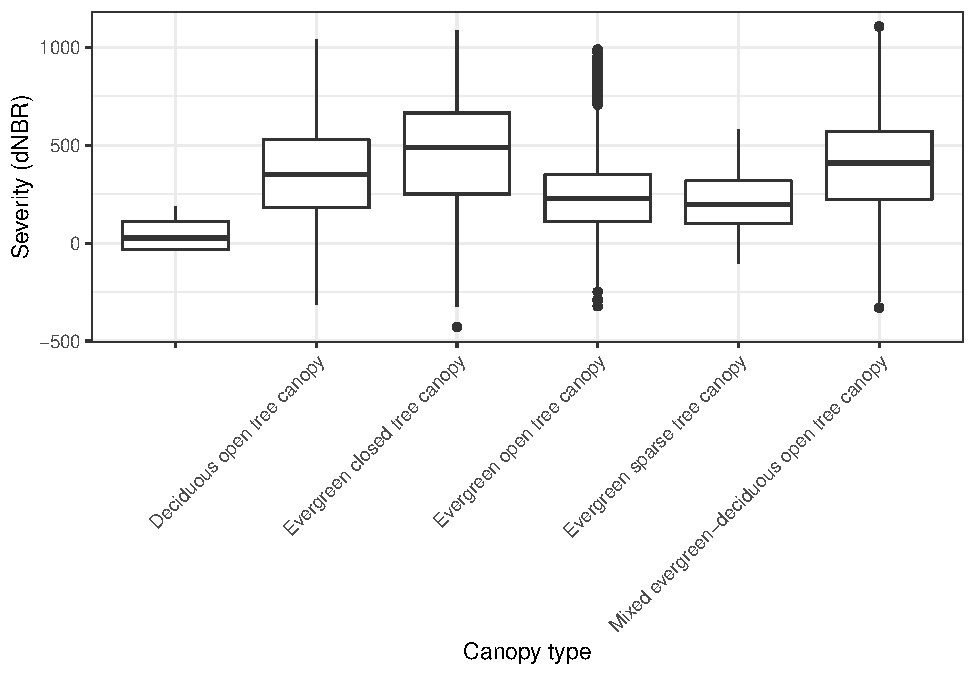
\includegraphics{term_project_files/figure-latex/ftypebarplot-1.pdf}

Bar plot of canopy categories

\begin{Shaded}
\begin{Highlighting}[]
\NormalTok{forest_topo }\OperatorTok\StringTok{ }
\StringTok{  }\KeywordTok{left_join}\NormalTok{(severity, }\DataTypeTok{by =} \StringTok{"severity_id"}\NormalTok{) }\OperatorTok\StringTok{ }
\StringTok{  }\KeywordTok{left_join}\NormalTok{(forest_risk, }\DataTypeTok{by =} \StringTok{"severity_id"}\NormalTok{) }\OperatorTok\StringTok{ }
\StringTok{  }\KeywordTok{select}\NormalTok{(dem, fri, severity) }\OperatorTok\StringTok{ }
\StringTok{  }\KeywordTok{ggplot}\NormalTok{(}\KeywordTok{aes}\NormalTok{(}\DataTypeTok{x =}\NormalTok{ dem, }\DataTypeTok{y =}\NormalTok{ severity, }\DataTypeTok{color =}\NormalTok{ fri)) }\OperatorTok{+}
\StringTok{  }\KeywordTok{geom_point}\NormalTok{(}\DataTypeTok{alpha =} \FloatTok{0.5}\NormalTok{) }\OperatorTok{+}
\StringTok{  }\KeywordTok{scale_color_viridis_c}\NormalTok{(}\DataTypeTok{option =} \StringTok{"magma"}\NormalTok{) }\OperatorTok{+}
\StringTok{  }\KeywordTok{labs}\NormalTok{(}\DataTypeTok{y =} \StringTok{"Severity (dNBR)"}\NormalTok{, }\DataTypeTok{x =} \StringTok{"Elevation (m)"}\NormalTok{) }\OperatorTok{+}
\StringTok{  }\KeywordTok{theme_light}\NormalTok{() }
\end{Highlighting}
\end{Shaded}

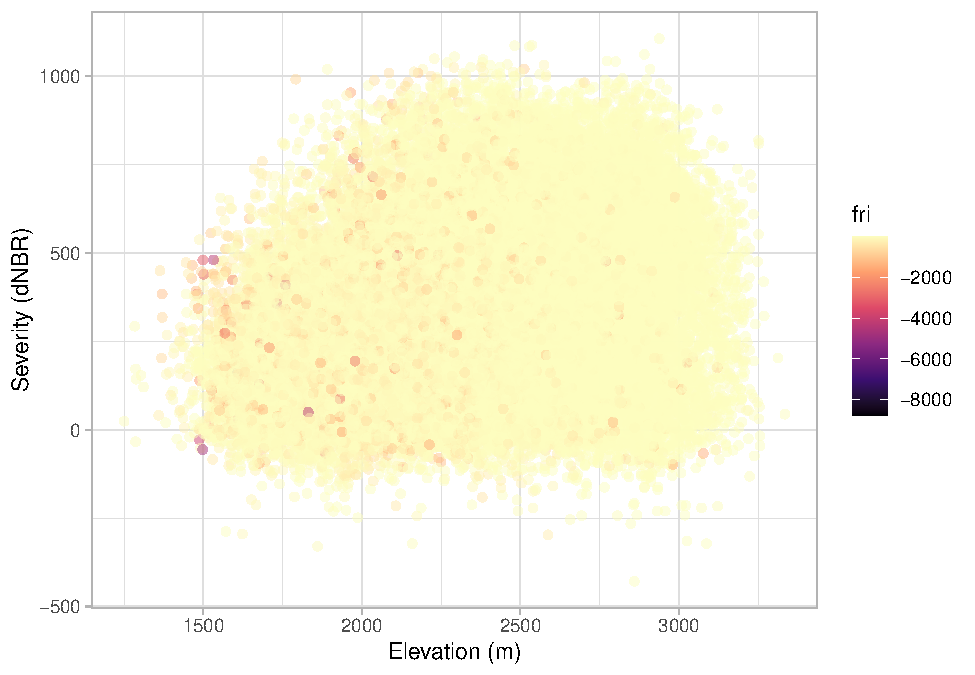
\includegraphics{term_project_files/figure-latex/risk_elevation-1.pdf}

Elevation x severity x fire risk index

\begin{Shaded}
\begin{Highlighting}[]
\NormalTok{forest_topo }\OperatorTok\StringTok{ }
\StringTok{  }\KeywordTok{left_join}\NormalTok{(severity, }\DataTypeTok{by =} \StringTok{"severity_id"}\NormalTok{) }\OperatorTok\StringTok{ }
\StringTok{  }\KeywordTok{left_join}\NormalTok{(forest_structure, }\DataTypeTok{by =} \StringTok{"severity_id"}\NormalTok{) }\OperatorTok\StringTok{ }
\StringTok{  }\KeywordTok{ggplot}\NormalTok{(}\KeywordTok{aes}\NormalTok{(}\DataTypeTok{x =}\NormalTok{ dem, }\DataTypeTok{y =}\NormalTok{ severity, }\DataTypeTok{color =}\NormalTok{ wwacc)) }\OperatorTok{+}
\StringTok{  }\KeywordTok{geom_point}\NormalTok{(}\DataTypeTok{alpha =} \FloatTok{0.5}\NormalTok{) }\OperatorTok{+}
\StringTok{  }\KeywordTok{scale_color_viridis_c}\NormalTok{(}\DataTypeTok{option =} \StringTok{"magma"}\NormalTok{) }\OperatorTok{+}
\StringTok{  }\KeywordTok{labs}\NormalTok{(}\DataTypeTok{y =} \StringTok{"Severity (dNBR)"}\NormalTok{, }\DataTypeTok{x =} \StringTok{"Elevation (m)"}\NormalTok{) }\OperatorTok{+}
\StringTok{  }\KeywordTok{theme_light}\NormalTok{() }
\end{Highlighting}
\end{Shaded}

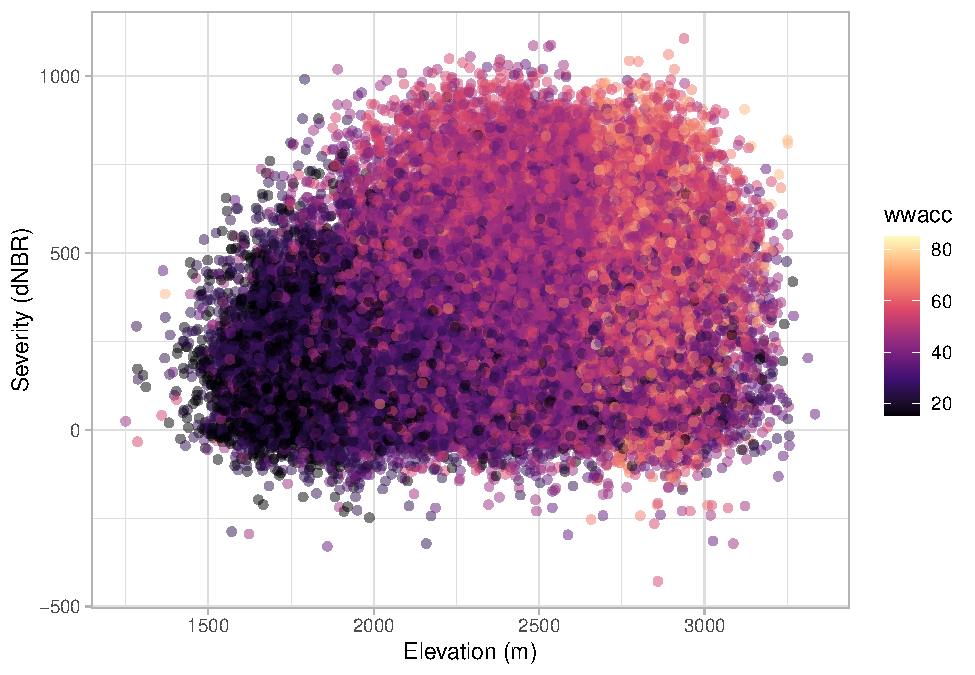
\includegraphics{term_project_files/figure-latex/cc_elevation-1.pdf}

Elevation x severity x canopy closure

\begin{Shaded}
\begin{Highlighting}[]
\NormalTok{forest_topo }\OperatorTok\StringTok{ }
\StringTok{  }\KeywordTok{left_join}\NormalTok{(severity, }\DataTypeTok{by =} \StringTok{"severity_id"}\NormalTok{) }\OperatorTok\StringTok{ }
\StringTok{  }\KeywordTok{left_join}\NormalTok{(forest_structure, }\DataTypeTok{by =} \StringTok{"severity_id"}\NormalTok{) }\OperatorTok\StringTok{ }
\StringTok{  }\KeywordTok{ggplot}\NormalTok{(}\KeywordTok{aes}\NormalTok{(}\DataTypeTok{x =}\NormalTok{ dem, }\DataTypeTok{y =}\NormalTok{ severity, }\DataTypeTok{color =}\NormalTok{ wwafuel40)) }\OperatorTok{+}
\StringTok{  }\KeywordTok{geom_point}\NormalTok{(}\DataTypeTok{alpha =} \FloatTok{0.5}\NormalTok{) }\OperatorTok{+}
\StringTok{  }\KeywordTok{scale_color_viridis_c}\NormalTok{(}\DataTypeTok{option =} \StringTok{"magma"}\NormalTok{) }\OperatorTok{+}
\StringTok{  }\KeywordTok{labs}\NormalTok{(}\DataTypeTok{y =} \StringTok{"Severity (dNBR)"}\NormalTok{, }\DataTypeTok{x =} \StringTok{"Elevation (m)"}\NormalTok{) }\OperatorTok{+}
\StringTok{  }\KeywordTok{theme_light}\NormalTok{()}
\end{Highlighting}
\end{Shaded}

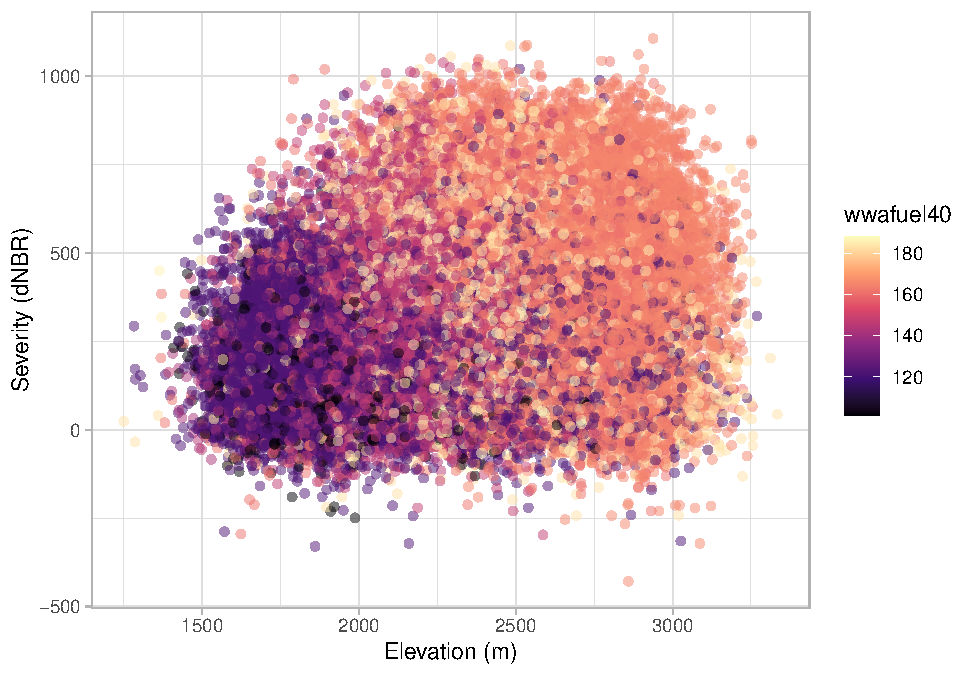
\includegraphics{term_project_files/figure-latex/fuels_elevation-1.pdf}

Elevation x severity x fuels40

Mean severity by vegetation type

\begin{Shaded}
\begin{Highlighting}[]
\NormalTok{forest_veg }\OperatorTok\StringTok{ }
\StringTok{  }\KeywordTok{pull}\NormalTok{(EVT) }\OperatorTok\StringTok{ }
\StringTok{  }\KeywordTok{unique}\NormalTok{()}
\end{Highlighting}
\end{Shaded}

\begin{verbatim}
##  [1] "Southern Rocky Mountain Mesic Montane Mixed Conifer Forest and Woodland"    
##  [2] "Rocky Mountain Aspen Forest and Woodland"                                   
##  [3] "Colorado Plateau Pinyon-Juniper Woodland"                                   
##  [4] "Rocky Mountain Subalpine Dry-Mesic Spruce-Fir Forest and Woodland"          
##  [5] "Southern Rocky Mountain Ponderosa Pine Woodland"                            
##  [6] "Inter-Mountain Basins Aspen-Mixed Conifer Forest and Woodland"              
##  [7] "Great Basin Pinyon-Juniper Woodland"                                        
##  [8] "Abies concolor Forest Alliance"                                             
##  [9] "Inter-Mountain Basins Curl-leaf Mountain Mahogany Woodland and Shrubland"   
## [10] "Rocky Mountain Bigtooth Maple Ravine Woodland"                              
## [11] "Rocky Mountain Lodgepole Pine Forest"                                       
## [12] "Southern Rocky Mountain Dry-Mesic Montane Mixed Conifer Forest and Woodland"
## [13] "Inter-Mountain Basins Juniper Savanna"                                      
## [14] "Rocky Mountain Montane Riparian Systems"                                    
## [15] "Inter-Mountain Basins Montane Riparian Systems"                             
## [16] "Rocky Mountain Subalpine-Montane Limber-Bristlecone Pine Woodland"          
## [17] "Recently Disturbed Developed Upland Deciduous Forest"                       
## [18] "Developed-Upland Deciduous Forest"                                          
## [19] "Rocky Mountain Foothill Limber Pine-Juniper Woodland"                       
## [20] "Middle Rocky Mountain Montane Douglas-fir Forest and Woodland"              
## [21] "Developed-Upland Mixed Forest"                                              
## [22] "Recently Disturbed Developed Upland Evergreen Forest"                       
## [23] "Developed-Upland Evergreen Forest"                                          
## [24] "Southern Rocky Mountain Ponderosa Pine Savanna"                             
## [25] "Western Great Plains Floodplain Systems"                                    
## [26] "Rocky Mountain Subalpine Mesic-Wet Spruce-Fir Forest and Woodland"          
## [27] "Inter-Mountain Basins Subalpine Limber-Bristlecone Pine Woodland"
\end{verbatim}

Lets check out the mean severity for each of these forest types.
The red dashed line is the high-severity threshold.
There are three forest types that have an average severity at or above the high-severity threshold of about 450 dNBR.
The three forest types are:

\begin{enumerate}
\def\labelenumi{\arabic{enumi}.}
\tightlist
\item
  Rocky Mountain Subalpine Dry-Mesic Spruce-Fir Forest and Woodland
\item
  Rocky Mountain Subalpine-Montane Limber-Bristlecone Pine Woodland
\item
  Southern Rocky Mountain Mesic Montane Mixed Conifer Forest and Woodland
\end{enumerate}

\begin{Shaded}
\begin{Highlighting}[]
\NormalTok{forest_veg }\OperatorTok\StringTok{ }
\StringTok{  }\KeywordTok{left_join}\NormalTok{(severity, }\DataTypeTok{by =} \StringTok{"severity_id"}\NormalTok{) }\OperatorTok\StringTok{ }
\StringTok{  }\KeywordTok{group_by}\NormalTok{(EVT) }\OperatorTok\StringTok{ }
\StringTok{  }\KeywordTok{summarise}\NormalTok{(}\DataTypeTok{mean_severity =} \KeywordTok{mean}\NormalTok{(severity, }\DataTypeTok{na.rm =} \OtherTok{TRUE}\NormalTok{)) }\OperatorTok\StringTok{ }
\StringTok{  }\KeywordTok{ggplot}\NormalTok{(}\KeywordTok{aes}\NormalTok{(}\DataTypeTok{x =}\NormalTok{ EVT, }\DataTypeTok{y =}\NormalTok{ mean_severity)) }\OperatorTok{+}
\StringTok{  }\KeywordTok{geom_hline}\NormalTok{(}\DataTypeTok{yintercept =} \DecValTok{450}\NormalTok{, }\DataTypeTok{linetype =} \StringTok{"dashed"}\NormalTok{, }\DataTypeTok{color =} \StringTok{"red"}\NormalTok{) }\OperatorTok{+}
\StringTok{  }\KeywordTok{geom_bar}\NormalTok{(}\DataTypeTok{stat =} \StringTok{"identity"}\NormalTok{) }\OperatorTok{+}
\StringTok{  }\KeywordTok{labs}\NormalTok{(}\DataTypeTok{x =} \StringTok{" "}\NormalTok{, }\DataTypeTok{y =} \StringTok{"Mean severity"}\NormalTok{) }\OperatorTok{+}
\StringTok{  }\KeywordTok{theme_bw}\NormalTok{() }\OperatorTok{+}
\StringTok{  }\KeywordTok{theme}\NormalTok{(}\DataTypeTok{axis.text.x =} \KeywordTok{element_text}\NormalTok{(}\DataTypeTok{angle =} \DecValTok{40}\NormalTok{, }\DataTypeTok{hjust =} \DecValTok{1}\NormalTok{)) }
\end{Highlighting}
\end{Shaded}

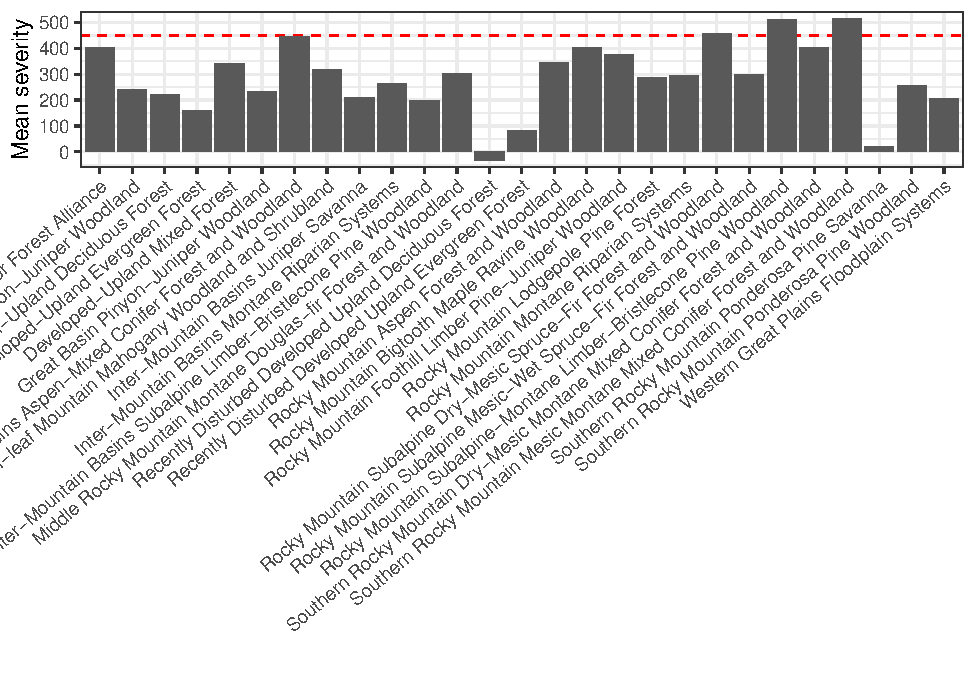
\includegraphics{term_project_files/figure-latex/vegtype_mean_sev-1.pdf}

\hypertarget{ggplot}{%
\chapter{Non-forest data visualization}\label{ggplot}}

Load packages

Simple scatter plot of non-forest severity vs.~elevation (m)

\begin{Shaded}
\begin{Highlighting}[]
\NormalTok{sev <-}\StringTok{ }\NormalTok{nf_topo }\OperatorTok\StringTok{ }
\StringTok{  }\KeywordTok{left_join}\NormalTok{(severity, }\DataTypeTok{by =} \StringTok{"severity_id"}\NormalTok{) }\OperatorTok\StringTok{ }
\StringTok{  }\KeywordTok{select}\NormalTok{(dem, severity)}

\NormalTok{reg <-}\StringTok{ }\KeywordTok{lm}\NormalTok{(}\DataTypeTok{formula=}\NormalTok{ severity }\OperatorTok{~}\StringTok{ }\NormalTok{dem, }\DataTypeTok{data =}\NormalTok{ sev)}
\NormalTok{regs <-}\StringTok{ }\KeywordTok{predict}\NormalTok{(reg, }\DataTypeTok{se.fit =} \OtherTok{TRUE}\NormalTok{)}
\NormalTok{regs <-}\StringTok{ }\KeywordTok{data.frame}\NormalTok{(}\DataTypeTok{mean =}\NormalTok{ regs}\OperatorTok{$}\NormalTok{fit,}
                    \DataTypeTok{upr =}\NormalTok{ regs}\OperatorTok{$}\NormalTok{fit }\OperatorTok{+}\StringTok{ }\FloatTok{1.96} \OperatorTok{*}\StringTok{ }\NormalTok{regs}\OperatorTok{$}\NormalTok{se.fit,}
                    \DataTypeTok{lwr =}\NormalTok{ regs}\OperatorTok{$}\NormalTok{fit }\OperatorTok{-}\StringTok{ }\FloatTok{1.96} \OperatorTok{*}\StringTok{ }\NormalTok{regs}\OperatorTok{$}\NormalTok{se.fit)}
            

\NormalTok{nf_topo }\OperatorTok\StringTok{ }
\StringTok{  }\KeywordTok{left_join}\NormalTok{(severity, }\DataTypeTok{by =} \StringTok{"severity_id"}\NormalTok{) }\OperatorTok\StringTok{ }
\StringTok{  }\KeywordTok{select}\NormalTok{(dem, severity) }\OperatorTok\StringTok{ }
\StringTok{  }\KeywordTok{ggplot}\NormalTok{(}\KeywordTok{aes}\NormalTok{(}\DataTypeTok{x =}\NormalTok{ dem, }\DataTypeTok{y =}\NormalTok{ severity, }\DataTypeTok{color=}\NormalTok{ dem)) }\OperatorTok{+}
\StringTok{  }\KeywordTok{geom_point}\NormalTok{(}\DataTypeTok{alpha =} \FloatTok{0.5}\NormalTok{) }\OperatorTok{+}
\StringTok{  }\KeywordTok{scale_color_viridis_c}\NormalTok{(}\DataTypeTok{option =} \StringTok{"magma"}\NormalTok{) }\OperatorTok{+}
\StringTok{  }\KeywordTok{geom_line}\NormalTok{(}\KeywordTok{aes}\NormalTok{(}\DataTypeTok{y =}\NormalTok{ regs}\OperatorTok{$}\NormalTok{mean, }\DataTypeTok{color =}\NormalTok{ regs}\OperatorTok{$}\NormalTok{mean)) }\OperatorTok{+}
\StringTok{  }\KeywordTok{labs}\NormalTok{(}\DataTypeTok{y =} \StringTok{"Severity (dNBR)"}\NormalTok{, }\DataTypeTok{x =} \StringTok{"Elevation (m)"}\NormalTok{) }\OperatorTok{+}
\StringTok{  }\KeywordTok{theme_light}\NormalTok{() }
\end{Highlighting}
\end{Shaded}

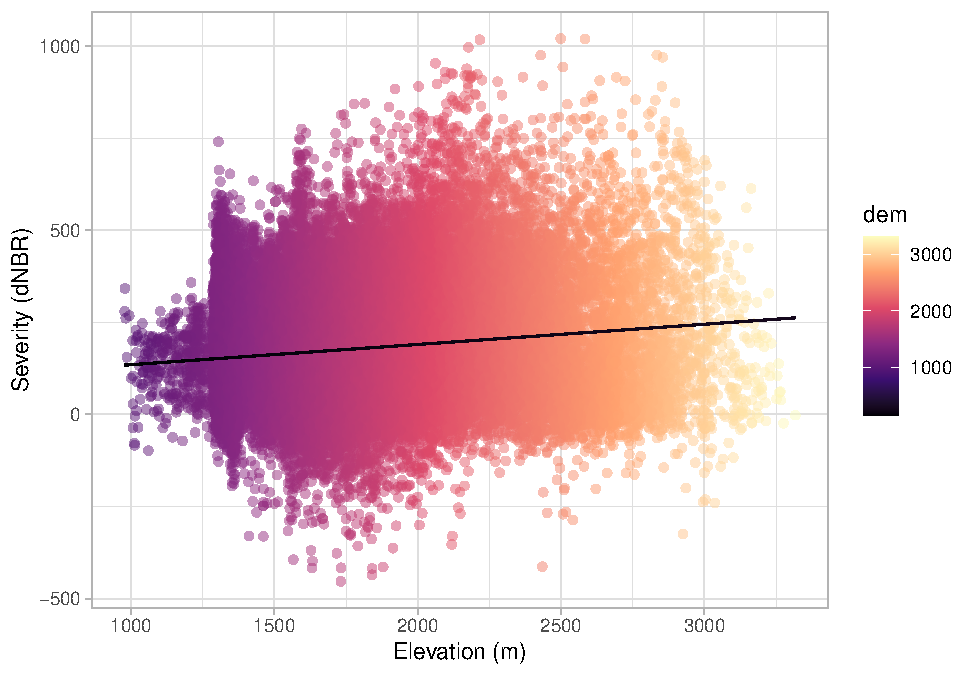
\includegraphics{term_project_files/figure-latex/nf_scatterplot-1.pdf}

\begin{Shaded}
\begin{Highlighting}[]
\NormalTok{nf_veg }\OperatorTok\StringTok{ }
\StringTok{  }\KeywordTok{left_join}\NormalTok{(severity, }\DataTypeTok{by =} \StringTok{"severity_id"}\NormalTok{) }\OperatorTok\StringTok{ }
\StringTok{  }\KeywordTok{filter}\NormalTok{(}\OperatorTok{!}\KeywordTok{is.na}\NormalTok{(severity_id)) }\OperatorTok\StringTok{ }
\StringTok{  }\KeywordTok{ggplot}\NormalTok{(}\KeywordTok{aes}\NormalTok{(}\DataTypeTok{x =}\NormalTok{ NVCSsubclass, }\DataTypeTok{y =}\NormalTok{ severity)) }\OperatorTok{+}
\StringTok{  }\KeywordTok{geom_boxplot}\NormalTok{() }\OperatorTok{+}
\StringTok{  }\KeywordTok{labs}\NormalTok{(}\DataTypeTok{y =} \StringTok{"Severity (dNBR)"}\NormalTok{, }\DataTypeTok{x =} \StringTok{"Canopy type"}\NormalTok{) }\OperatorTok{+}
\StringTok{  }\KeywordTok{theme_bw}\NormalTok{() }\OperatorTok{+}
\StringTok{  }\KeywordTok{theme}\NormalTok{(}\DataTypeTok{axis.text.x =} \KeywordTok{element_text}\NormalTok{(}\DataTypeTok{angle =} \DecValTok{45}\NormalTok{, }\DataTypeTok{hjust =} \DecValTok{1}\NormalTok{)) }
\end{Highlighting}
\end{Shaded}

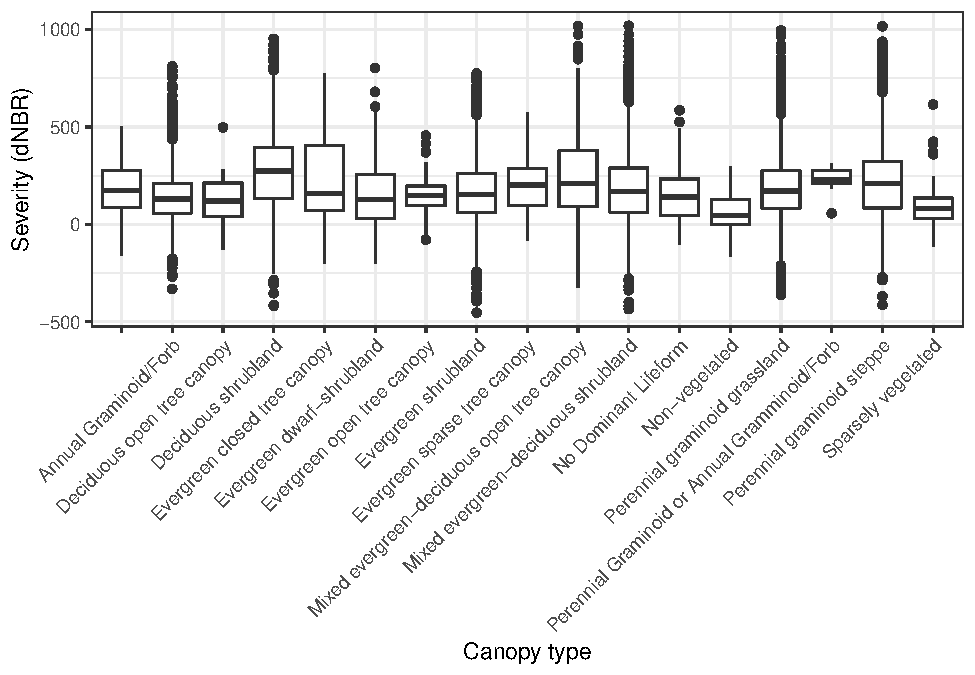
\includegraphics{term_project_files/figure-latex/nf_barplot-1.pdf}

Bar plot of non-forest canopy categories.

\begin{Shaded}
\begin{Highlighting}[]
\NormalTok{nf_topo }\OperatorTok\StringTok{ }
\StringTok{  }\KeywordTok{left_join}\NormalTok{(severity, }\DataTypeTok{by =} \StringTok{"severity_id"}\NormalTok{) }\OperatorTok\StringTok{ }
\StringTok{  }\KeywordTok{left_join}\NormalTok{(nf_risk, }\DataTypeTok{by =} \StringTok{"severity_id"}\NormalTok{) }\OperatorTok\StringTok{ }
\StringTok{  }\KeywordTok{select}\NormalTok{(dem, fri, severity) }\OperatorTok\StringTok{ }
\StringTok{  }\KeywordTok{ggplot}\NormalTok{(}\KeywordTok{aes}\NormalTok{(}\DataTypeTok{x =}\NormalTok{ dem, }\DataTypeTok{y =}\NormalTok{ severity, }\DataTypeTok{color =}\NormalTok{ fri)) }\OperatorTok{+}
\StringTok{  }\KeywordTok{geom_point}\NormalTok{(}\DataTypeTok{alpha =} \FloatTok{0.5}\NormalTok{) }\OperatorTok{+}
\StringTok{  }\KeywordTok{scale_color_viridis_c}\NormalTok{(}\DataTypeTok{option =} \StringTok{"magma"}\NormalTok{) }\OperatorTok{+}
\StringTok{  }\KeywordTok{labs}\NormalTok{(}\DataTypeTok{y =} \StringTok{"Severity (dNBR)"}\NormalTok{, }\DataTypeTok{x =} \StringTok{"Elevation (m)"}\NormalTok{) }\OperatorTok{+}
\StringTok{  }\KeywordTok{theme_light}\NormalTok{() }
\end{Highlighting}
\end{Shaded}

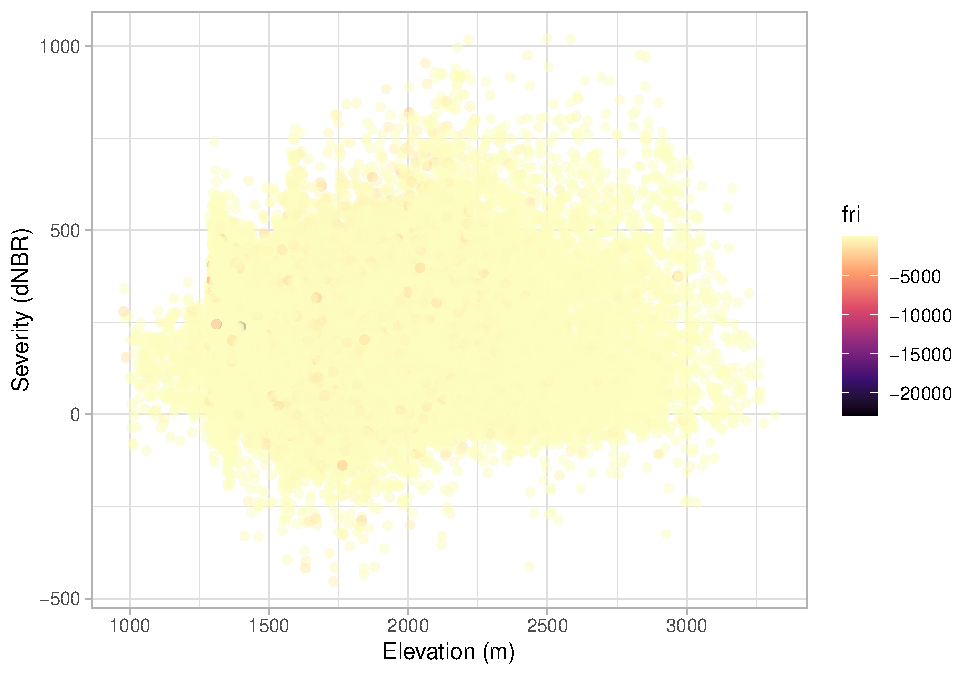
\includegraphics{term_project_files/figure-latex/nf_risk_elevation-1.pdf}

Elevation x severity x fire risk index

\begin{Shaded}
\begin{Highlighting}[]
\NormalTok{nf_topo }\OperatorTok\StringTok{ }
\StringTok{  }\KeywordTok{left_join}\NormalTok{(severity, }\DataTypeTok{by =} \StringTok{"severity_id"}\NormalTok{) }\OperatorTok\StringTok{ }
\StringTok{  }\KeywordTok{left_join}\NormalTok{(nf_structure, }\DataTypeTok{by =} \StringTok{"severity_id"}\NormalTok{) }\OperatorTok\StringTok{ }
\StringTok{  }\KeywordTok{ggplot}\NormalTok{(}\KeywordTok{aes}\NormalTok{(}\DataTypeTok{x =}\NormalTok{ dem, }\DataTypeTok{y =}\NormalTok{ severity, }\DataTypeTok{color =}\NormalTok{ wwacc)) }\OperatorTok{+}
\StringTok{  }\KeywordTok{geom_point}\NormalTok{(}\DataTypeTok{alpha =} \FloatTok{0.5}\NormalTok{) }\OperatorTok{+}
\StringTok{  }\KeywordTok{scale_color_viridis_c}\NormalTok{(}\DataTypeTok{option =} \StringTok{"magma"}\NormalTok{) }\OperatorTok{+}
\StringTok{  }\KeywordTok{labs}\NormalTok{(}\DataTypeTok{y =} \StringTok{"Severity (dNBR)"}\NormalTok{, }\DataTypeTok{x =} \StringTok{"Elevation (m)"}\NormalTok{) }\OperatorTok{+}
\StringTok{  }\KeywordTok{theme_light}\NormalTok{() }
\end{Highlighting}
\end{Shaded}

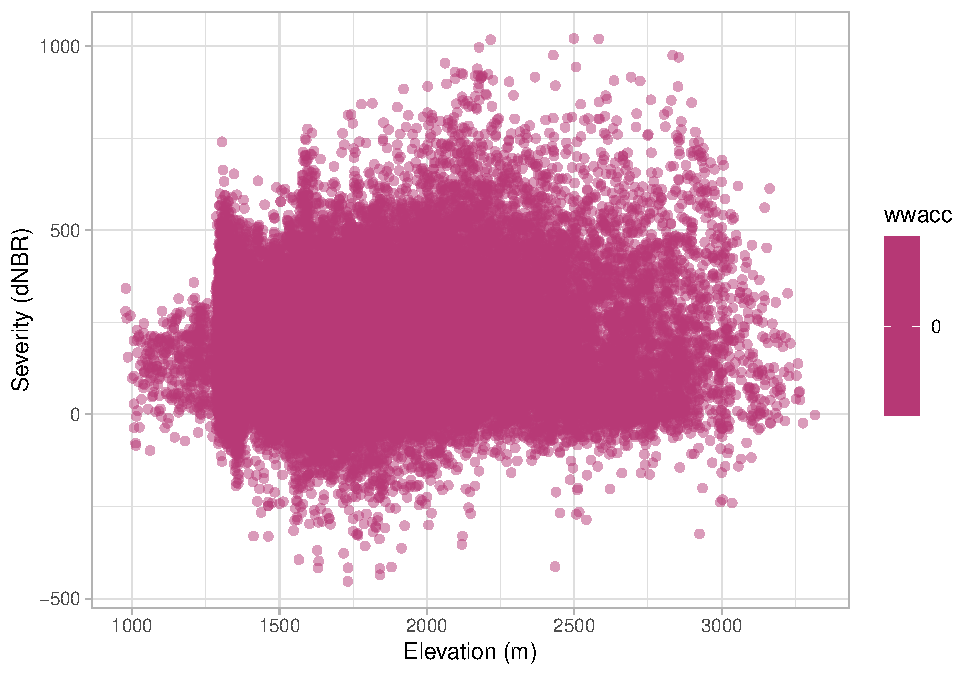
\includegraphics{term_project_files/figure-latex/nf_cc_elevation-1.pdf}

Elevation x severity x canopy closure. This figures illustrates that non-forest landcover has no discernable canopy.

\begin{Shaded}
\begin{Highlighting}[]
\NormalTok{nf_topo }\OperatorTok\StringTok{ }
\StringTok{  }\KeywordTok{left_join}\NormalTok{(severity, }\DataTypeTok{by =} \StringTok{"severity_id"}\NormalTok{) }\OperatorTok\StringTok{ }
\StringTok{  }\KeywordTok{left_join}\NormalTok{(nf_structure, }\DataTypeTok{by =} \StringTok{"severity_id"}\NormalTok{) }\OperatorTok\StringTok{ }
\StringTok{  }\KeywordTok{ggplot}\NormalTok{(}\KeywordTok{aes}\NormalTok{(}\DataTypeTok{x =}\NormalTok{ dem, }\DataTypeTok{y =}\NormalTok{ severity, }\DataTypeTok{color =}\NormalTok{ wwafuel40)) }\OperatorTok{+}
\StringTok{  }\KeywordTok{geom_point}\NormalTok{(}\DataTypeTok{alpha =} \FloatTok{0.5}\NormalTok{) }\OperatorTok{+}
\StringTok{  }\KeywordTok{scale_color_viridis_c}\NormalTok{(}\DataTypeTok{option =} \StringTok{"magma"}\NormalTok{) }\OperatorTok{+}
\StringTok{  }\KeywordTok{labs}\NormalTok{(}\DataTypeTok{y =} \StringTok{"Severity (dNBR)"}\NormalTok{, }\DataTypeTok{x =} \StringTok{"Elevation (m)"}\NormalTok{) }\OperatorTok{+}
\StringTok{  }\KeywordTok{theme_light}\NormalTok{()}
\end{Highlighting}
\end{Shaded}

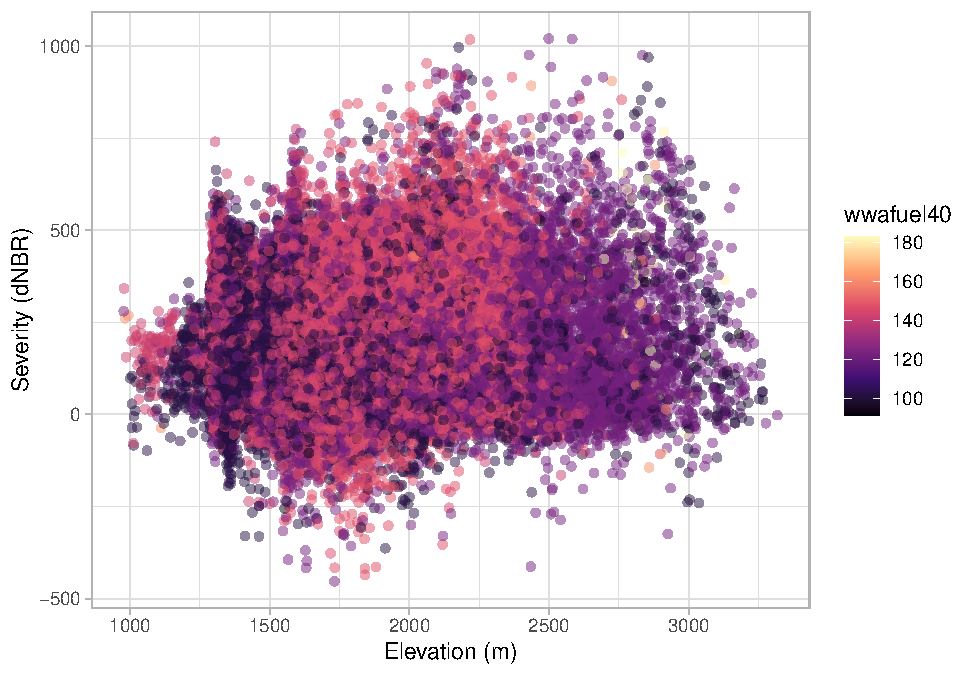
\includegraphics{term_project_files/figure-latex/nf_fuels_elevation-1.pdf}

Elevation x severity x fuels40

Mean severity by vegetation type

\begin{Shaded}
\begin{Highlighting}[]
\NormalTok{nf_veg }\OperatorTok\StringTok{ }
\StringTok{  }\KeywordTok{pull}\NormalTok{(EVT) }\OperatorTok\StringTok{ }
\StringTok{  }\KeywordTok{unique}\NormalTok{()}
\end{Highlighting}
\end{Shaded}

\begin{verbatim}
##  [1] "Inter-Mountain Basins Mixed Salt Desert Scrub"                              
##  [2] "Rocky Mountain Gambel Oak-Mixed Montane Shrubland"                          
##  [3] "Herbaceous Semi-dry"                                                        
##  [4] "Inter-Mountain Basins Big Sagebrush Shrubland"                              
##  [5] "Introduced Upland Vegetation-Annual Grassland"                              
##  [6] "Artemisia tridentata ssp. vaseyana Shrubland Alliance"                      
##  [7] "NASS-Fallow/Idle Cropland"                                                  
##  [8] "Sonora-Mojave Semi-Desert Chaparral"                                        
##  [9] "Inter-Mountain Basins Big Sagebrush Steppe"                                 
## [10] "Quercus gambelii Shrubland Alliance"                                        
## [11] "Colorado Plateau Mixed Low Sagebrush Shrubland"                             
## [12] "Inter-Mountain Basins Greasewood Flat"                                      
## [13] "Rocky Mountain Subalpine-Montane Mesic Meadow"                              
## [14] "Great Basin Xeric Mixed Sagebrush Shrubland"                                
## [15] "NASS-Close Grown Crop"                                                      
## [16] "Inter-Mountain Basins Semi-Desert Shrub-Steppe"                             
## [17] "Colorado Plateau Pinyon-Juniper Woodland"                                   
## [18] "Rocky Mountain Foothill Limber Pine-Juniper Woodland"                       
## [19] "Inter-Mountain Basins Semi-Desert Grassland"                                
## [20] "Inter-Mountain Basins Montane Sagebrush Steppe"                             
## [21] "Great Basin Semi-Desert Chaparral"                                          
## [22] "Inter-Mountain Basins Aspen-Mixed Conifer Forest and Woodland"              
## [23] "Developed-Upland Shrubland"                                                 
## [24] "Agriculture-Pasture and Hay"                                                
## [25] "Rocky Mountain Lower Montane-Foothill Shrubland"                            
## [26] "Recently Disturbed Pasture and Hayland"                                     
## [27] "Introduced Upland Vegetation-Perennial Grassland and Forbland"              
## [28] "Developed-Upland Herbaceous"                                                
## [29] "Inter-Mountain Basins Curl-leaf Mountain Mahogany Woodland and Shrubland"   
## [30] "Abies concolor Forest Alliance"                                             
## [31] "North American Warm Desert Riparian Systems"                                
## [32] "Colorado Plateau Blackbrush-Mormon-tea Shrubland"                           
## [33] "Introduced Upland Vegetation-Annual and Biennial Forbland"                  
## [34] "Barren"                                                                     
## [35] "Columbia Plateau Low Sagebrush Steppe"                                      
## [36] "Inter-Mountain Basins Juniper Savanna"                                      
## [37] "Wyoming Basins Dwarf Sagebrush Shrubland and Steppe"                        
## [38] "Developed-Roads"                                                            
## [39] "Mojave Mid-Elevation Mixed Desert Scrub"                                    
## [40] "Coleogyne ramosissima Shrubland Alliance"                                   
## [41] "Southern Rocky Mountain Mesic Montane Mixed Conifer Forest and Woodland"    
## [42] "Rocky Mountain Alpine/Montane Sparsely Vegetated Systems"                   
## [43] "Inter-Mountain Basins Mat Saltbush Shrubland"                               
## [44] "Great Basin Pinyon-Juniper Woodland"                                        
## [45] "Southern Rocky Mountain Montane-Subalpine Grassland"                        
## [46] "Arctostaphylos patula Shrubland Alliance"                                   
## [47] "Rocky Mountain Subalpine Dry-Mesic Spruce-Fir Forest and Woodland"          
## [48] "Inter-Mountain Basins Sparsely Vegetated Systems"                           
## [49] "Mogollon Chaparral"                                                         
## [50] "Columbia Plateau Steppe and Grassland"                                      
## [51] "Herbaceous Wetlands"                                                        
## [52] "Rocky Mountain Montane Riparian Systems"                                    
## [53] "Quarries-Strip Mines-Gravel Pits"                                           
## [54] "Rocky Mountain Alpine Dwarf-Shrubland"                                      
## [55] "Introduced Riparian Vegetation"                                             
## [56] "Southern Rocky Mountain Dry-Mesic Montane Mixed Conifer Forest and Woodland"
## [57] "Southern Colorado Plateau Sand Shrubland"                                   
## [58] "Recently Burned-Herb and Grass Cover"                                       
## [59] "Open Water"                                                                 
## [60] "NASS-Row Crop"                                                              
## [61] "Sonora-Mojave Creosotebush-White Bursage Desert Scrub"                      
## [62] "Recently Disturbed Developed Upland Shrubland"                              
## [63] "Agriculture-Cultivated Crops and Irrigated Agriculture"                     
## [64] "Southern Rocky Mountain Ponderosa Pine Woodland"                            
## [65] "Rocky Mountain Subalpine/Upper Montane Riparian Systems"
\end{verbatim}

Lets check out the mean severity for each of these forest types.
The red dashed line is the high-severity threshold.

\begin{Shaded}
\begin{Highlighting}[]
\NormalTok{nf_veg }\OperatorTok\StringTok{ }
\StringTok{  }\KeywordTok{left_join}\NormalTok{(severity, }\DataTypeTok{by =} \StringTok{"severity_id"}\NormalTok{) }\OperatorTok\StringTok{ }
\StringTok{  }\KeywordTok{group_by}\NormalTok{(EVT) }\OperatorTok\StringTok{ }
\StringTok{  }\KeywordTok{summarise}\NormalTok{(}\DataTypeTok{mean_severity =} \KeywordTok{mean}\NormalTok{(severity, }\DataTypeTok{na.rm =} \OtherTok{TRUE}\NormalTok{)) }\OperatorTok\StringTok{ }
\StringTok{  }\KeywordTok{ggplot}\NormalTok{(}\KeywordTok{aes}\NormalTok{(}\DataTypeTok{x =}\NormalTok{ EVT, }\DataTypeTok{y =}\NormalTok{ mean_severity)) }\OperatorTok{+}
\StringTok{  }\KeywordTok{geom_hline}\NormalTok{(}\DataTypeTok{yintercept =} \DecValTok{450}\NormalTok{, }\DataTypeTok{linetype =} \StringTok{"dashed"}\NormalTok{, }\DataTypeTok{color =} \StringTok{"red"}\NormalTok{) }\OperatorTok{+}
\StringTok{  }\KeywordTok{geom_bar}\NormalTok{(}\DataTypeTok{stat =} \StringTok{"identity"}\NormalTok{) }\OperatorTok{+}
\StringTok{  }\KeywordTok{labs}\NormalTok{(}\DataTypeTok{x =} \StringTok{" "}\NormalTok{, }\DataTypeTok{y =} \StringTok{"Mean severity"}\NormalTok{) }\OperatorTok{+}
\StringTok{  }\KeywordTok{theme_bw}\NormalTok{() }\OperatorTok{+}
\StringTok{  }\KeywordTok{theme}\NormalTok{(}\DataTypeTok{axis.text.x =} \KeywordTok{element_text}\NormalTok{(}\DataTypeTok{angle =} \DecValTok{40}\NormalTok{, }\DataTypeTok{hjust =} \DecValTok{1}\NormalTok{)) }
\end{Highlighting}
\end{Shaded}

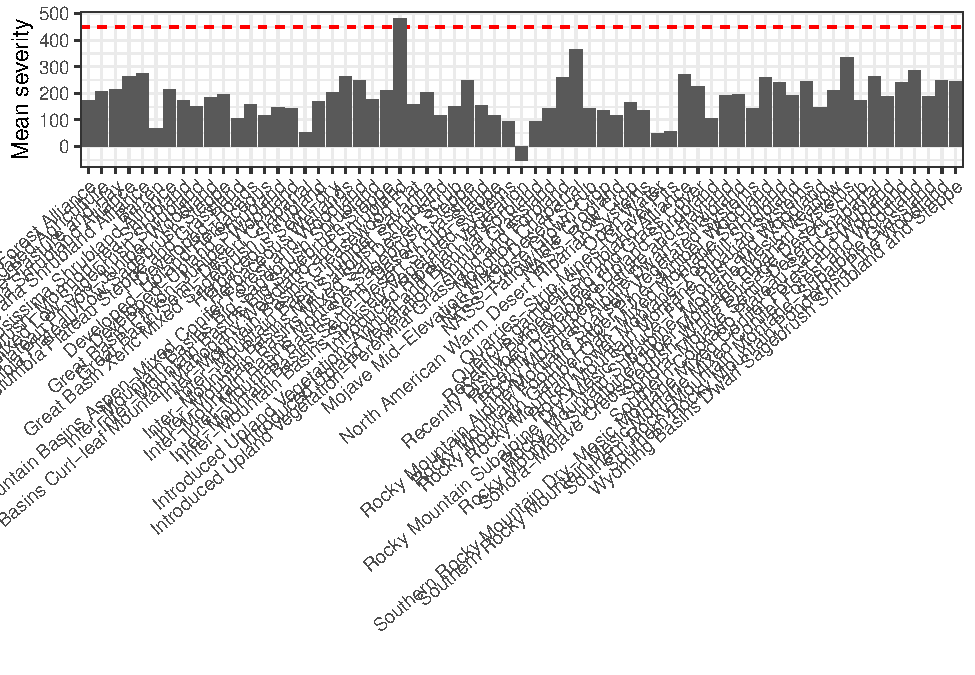
\includegraphics{term_project_files/figure-latex/nf_vegtype_mean_sev-1.pdf}

\bibliography{book.bib,packages.bib}

\end{document}
